\chapter{Introduction}\label{introduction}
%\doublespacing

%The term 'jet' was first introduced by \citet{baade54} to the extended knotty structure of M87.
Jets from Active Galactic Nuclei (AGN) are collimated streams of magnetized plasma emanating from the centre of the AGN near the supermassive black hole (SMBH) at speeds close to the speed of light. They form large plumes or lobe structures extending tens to several hundreds of kilo parsecs in the intergalactic medium or intracluster medium (ICM). Many giant elliptical galaxies harbour SMBH (their typical mass being $\sim 10^5 - 10^{10} \rm \ M_{\odot}$) at their centres and it is now believed that accretion onto the SMBH powers the bipolar jets. The fraction of galaxies that host radio-loud AGN is a sensitive function of the galaxy mass and for the central bright elliptical galaxies of galaxy clusters the fraction exceeds 30\%{} \citep{best05}. The jets emanating from the central radio galaxies in clusters are also thought to be responsible for balancing the cooling of the ICM and preventing the occurrence of massive accretion flows of cooled gas (cooling flows). The AGN in a cluster therefore functions like a thermostat, regulating the cluster gas temperature, keeping it nearly isothermal at $\approx{}10^{7-8}$ K \citep{fabian05}.

Morphologically AGN radio sources are classified into two groups: i) Edge-darkened Fanaroff-Riley I (FRI) sources and ii) Edge-brightened Fanaroff-Riley II (FRII) sources. The lower-powered FRI sources have bright radio jets near the core which quickly decelerate and flare out to form large plumes. The deceleration and the turbulent transition of the jet can be caused by recollimation shocks and entrainment of the ambient medium by the jets \citep{bicknell84}. Interaction of the jet with ambient clouds is another potential cause of jet deceleration \citep{perucho14}. On the other hand, higher-powered FRII jets remain supersonic and collimated and produce hot spots at the edge of the source. The division in jet power between FRI and FRII sources lies at approximately $\sim10^{43}$ erg s$^{-1}$ \citep{bicknell95, ledlow96} although there are sources of either class on either side of the divide. The precise reasons for the two morphological types of radio sources is not fully understood, but the rate of deceleration of the jets as they propagate through the ambient medium is an important factor \citep{bicknell95, kawakatu09}.

To understand the morphology of radio jets, lobes, and plumes on tens to hundreds of kpc scales it is vital to understand the energetics, composition of the jet and the dynamical interaction of the jet with the ISM/ICM near its origin. In this thesis, I present detailed models of knot formation and radial oscillations of Hydra jets (in particular, the northern jet) in the central 10~kpc of Hydra A radio source. Combining this with a careful extrapolation of the ICM thermodynamic profile toward the core and a proper estimate of the pressure in the jet-fed lobe, I constrain the power, composition, density, and velocity of the jet near its origin. The constrained jet parameters are then used in three dimensional precessing jet simulations to understand the physics of the inner 20~kpc of the northern jet and constrain the precession period and precession angle. The results from this multifaceted approach provide a new reliable basis from which to perform large-scale simulations and understand mechanisms of energy and mass transport by AGN jets, and the inhibition of cooling flows in the ICM.

%I have undertaken a detailed examination and modelling of the knot formation and radius oscillations of the jet in the central 10 kpc of the Hydra A radio jets.

\section{Bright knots}

\begin{figure*}
\centering
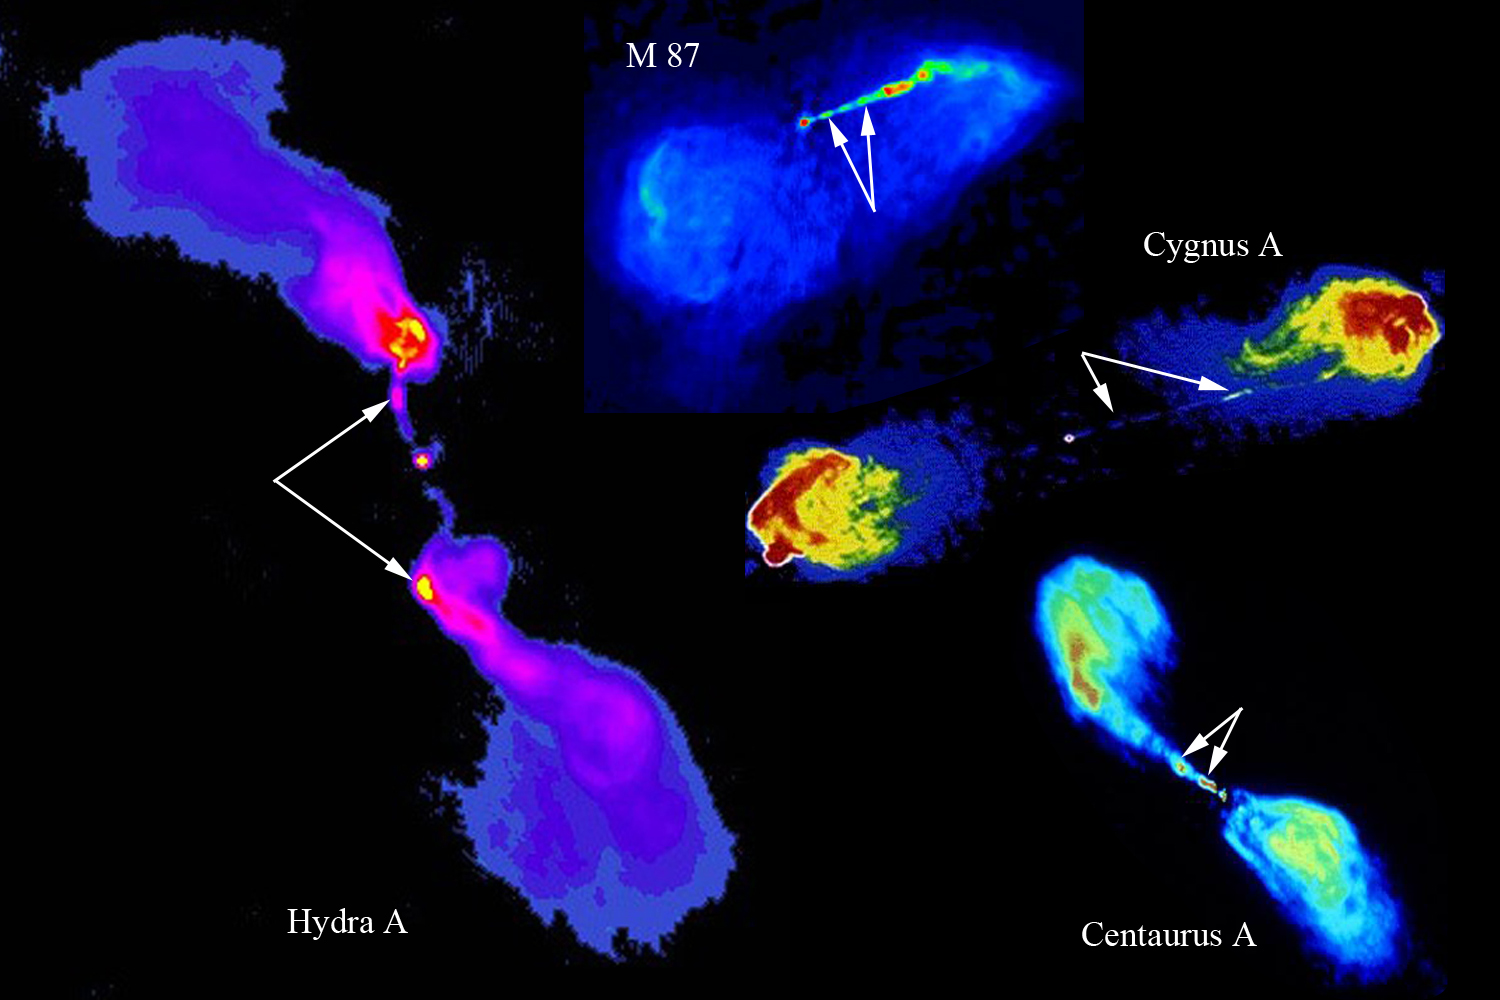
\includegraphics[width=\linewidth]{bright_knots.jpg}
\caption{VLA image of a) Hydra A \citep{taylor90}, b) M87 citep{owen}, c) Cygnus A jets. Bright knots, several of which are highlighted with arrows, can be clearly seen along the collimated jet.}
\label{knot}
\end{figure*}


Bright knots are a prominent feature in many classical AGN jets, for example, M87\citep{owen89}, Cygnus A \citep{steenbrugge07}, Centaurus A \citep{goodger10}, and the spectacular source, Hydra A,  which exhibits a high degree of S-symmetry of its structure \citep{taylor90} (see Fig.~\ref{knot}). However, to date, the mechanism of the formation of the knots is not clearly understood. Although a number of theories have been developed to explain these bright knots, they are restricted to explain particular sources. In this section I discuss the theories of the formation of bright knots.

\subsection{Shock by velocity variation}
The first theoretical explanation for the bright knots in astrophysical jets was proposed by \citet{rees78}, who interpreted the bright knots of M87 as enhanced synchrotron emission from shocks resulting from a variable flow velocity. The conditions for the formation of shock waves in this theory are 1) that a faster region of the jet plasma overtakes an older and slower region, and 2) that the relative velocities are supersonic.  

%% aln  write more about this model


% Complication in the modelling of the variation in the blob velocity and the ejection interval of blobs makes this model difficult for numerical modelling. 
% This model is used 

\subsection{Jet-cloud interaction}
\citet{blandford79} presented an alternative shock model for the explanation of the knots of M87. According to their model the supersonic M87 jet hits dense interstellar clouds of sufficiently large size along its path. This collision results in bow shaped shocks behind the cloud. The shock accelerated jet plasma downstream of the shocks are responsible for the bright knots. Using numerical models \citet{coleman85} later modelled the interaction of a supersonic jet with a cylindrical cloud and showed that a bow shock is created at the impact region. They also explained the optical spectral index of the knots with this model.  

%This model is criticised for the short lifetime of the shocks relative to the age of the knots \citep{goodger10}

\subsection{Shocks by Kelvin-Helmholtz (KH) instabilities}
 \citet{bicknell96} proposed another shock model for the formation of the knots of M87 jet. They proposed that the bright knots in M87 are oblique shocks produced by helical modes of the KH instability, produced when a lighter jet interacts with the ambient medium. The increasing brightness of the knots with distance form the black hole was attributed to the increase in the shock strength due to the growth of the KH instability. They also showed that for a relativistic jet with Lorentz factor $\Gamma=5$ -- 7, the velocity of the shocks is consistent with the pattern speed of the bright knots. 

\subsection{Plasmon model}
The bright knots of AGN jets have also been modelled as blobs of magnetised plasma, plasmons, ejected periodically from the central black hole \citep{shklovskii77, shklovskii80}. The plasmons of mass $\approx$~0.1$M_{\odot}$ move with a relativistic velocity $\beta >0.65$ through the dense ambient medium. Deceleration of the plasmons by the interaction with the ambient medium constantly accelerates the electrons within the cloud and forms the bright knots.  

This model was used to interpret the moving knots of the superluminal quasar 3C 345 \citep{qian92}. Because of the motion of the knots, the plasmon model is also popular in the interpretation of observations of some protostellar jets \citep{goodson97} and VLBI AGN jets \citep{hough13}.

%\subsubsection{Othern models} Few other models have been proposed to explain bright knots in astrophysical jets. For example, \citep{lapenta05} explained the bright knots as a train of magnetic bubbles.


\subsection{Reconfinement shock model}\label{sec:reconf}
%This is one of the first models of bright knots in jets proposed by \citep{norman82}. According to this model the bright knots are results of quasi-steady periodic reconfinement shocks produced when the supersonic jet interacts with the ambient medium. 

%\begin{figure}[h!]
%\centering
%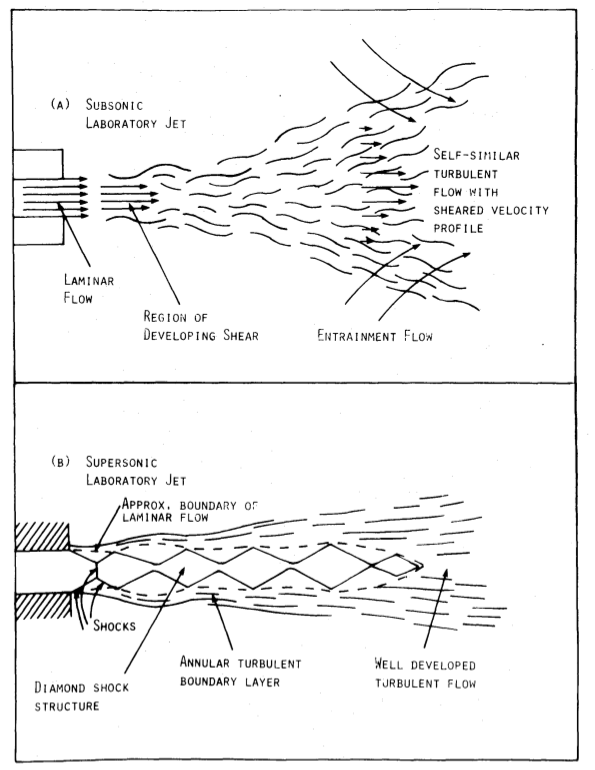
\includegraphics[width=\linewidth]{ifd.png}
%\caption{\noteA{replace this figure and amend caption and text accordingly.} A schematic diagram showing the structural difference of subsonic (panel A) and supersonic (panel B) flow. A subsonic flow is never collimated and the jet gradually forms a self-similar turbulent flow. However a supersonic flow is immediately recollimated by reconfinement shocks, marked here by solid diamond shaped lines and therefore also referred to as ``diamond shocks'', and continues as a laminar flow until it becomes subsonic. This image is taken from \citet{bicknell84}.}
%\label{fd}
%\end{figure}

\begin{figure}[h!]
\centering
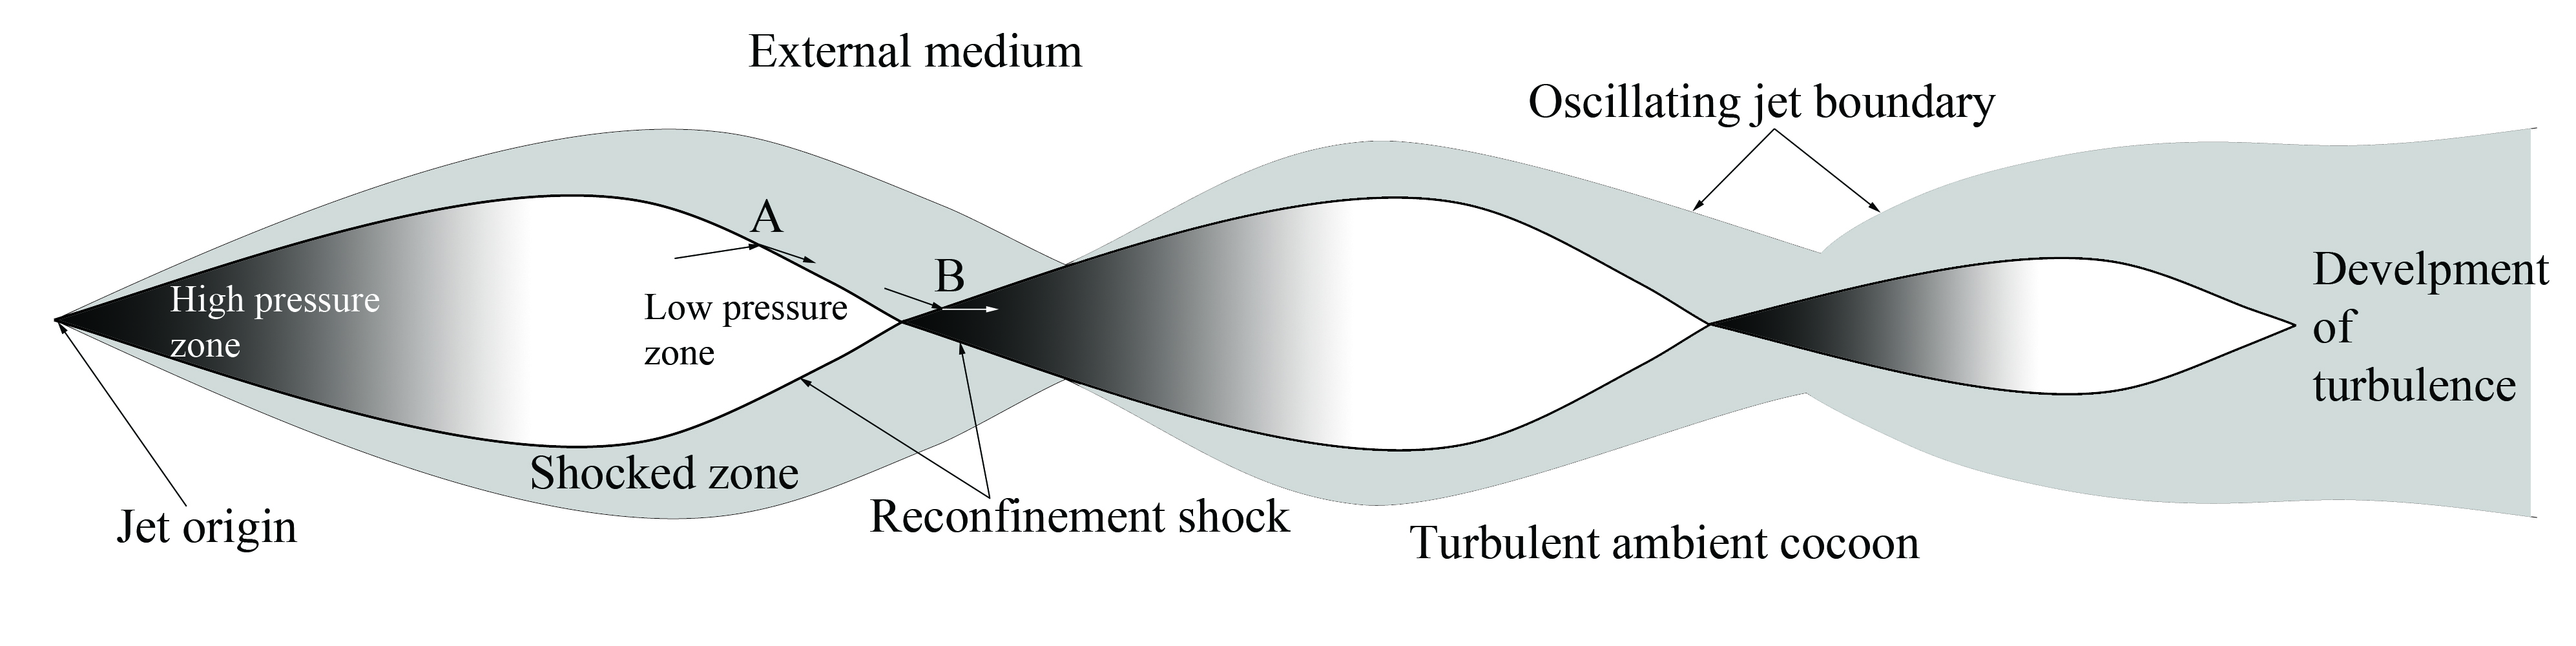
\includegraphics[width=\linewidth]{rsh.jpg}
\caption{Structures developed near the base of a supersonic jet. The initial over pressured jet (marked by high pressure zone) expands freely in the environment. It quickly reaches pressure equilibrium, over-expands and collimated by the external pressure via a reconfinement shock. The change in flow direction caused by the reconfinement shocks are shown in two zones A and B. The reconfinement shock converges towards the jet axis to form a biconical shock structure. The recollimated jet becomes over-pressured again and the cycle repeats. The jet boundary follow the oscillations of the reconfinement shocks. Shock deceleration by a number of biconical shock makes the jet subsonic and a turbulence gradually develops.}
\label{fig:rsh}
\end{figure}

The structures of reconfinement shocks in supersonic flows were first observed in laboratory jets more than a century ago (see \citet{krehl09} for the history of supersonic laboratory jets). When a supersonic jet interacts with its surroundings, the dynamics of the jet is affected by the external pressure. Fig.~\ref{fig:rsh} shows the structures developed near the base of a supersonic jet. The initially over-pressured jet (marked by high pressure zone) expands freely in the ambient medium. It soon reaches pressure equilibrium with the environment and is recollimated by the ambient pressure. Since the jet is supersonic the recollimation occurs through reconfinement shocks.
The reconfinement shocks change the flow direction as indicated in point A and B. The recollimated jet becomes overpressured again and the cycle repeats. The reconfinement shocks periodically converge to either: i) points on the jet axis to form biconical shocks if the jet is only slightly over-pressured with respect to the ambient medium or, ii) planar shocks, known as Mach disks, transverse to the flow if the jet is highly over-pressured. The jet boundary also oscillates following the oscillation of the reconfinement shocks (see Fig.~\ref{fig:rsh}).


%% aln the jet terminal hot-spot and the radio lobes had been predicted by Scheuer and Blandford and Rees. Norman et al confirmed this. 
\citet{norman82} first drew attention to the reconfinement shocks as an explanation for the bright knots of AGN jets. With a 2D hydrodynamical numerical model they explored the structures of a supersonic jet- i) reconfiment shocks along the jet, ii) A working surface at the end of the jet, iii) a cocoon. They argued that these structures could be the possible explanation for the following features of astrophysical jets respectively- i) bright knots ii) hot spots at the edge of the source iii) radio lobes. Subsequently, \citet{falle85} showed (qualitatively) that the spacings of reconfinement shocks of numerical jet model closely matches with the knot spacing of M87. The reconfinement shock model has also been well explored in analytical form \citep{canto89, kaiser97, komissarov97}. \citet{stawarz06}, for example, showed analytically that the HST 1 bright knot of M87 is a reconfinement shock. From the study presented in this thesis it becomes clear that the bright knots of the Hydra A northern jet are clearly a consequence of reconfinement shocks that appear naturally in hydrodynamic models. 

Interpreting bright knots as periodic reconfinement shocks is further motivated by the theoretical relationship for the natural wavelength of a supersonic jet described in \citet{birkhoff57a}. According to this relationship, the natural wavelength $\Lambda$ of a non-relativistic supersonic jet radius $r_{\rm jet}$ and Mach number $M$, in near pressure equilibrium is given by
 \begin{equation}
\Lambda/r_{\rm jet} \approx 2.6 \sqrt{M^2 - 1}
\label{e:birkhoff}
\end{equation}
%The Mach number is related to the velocity and density parameter of the jet \citep{bicknell94a}:
%\begin{equation}
%M = (2+ 3\chi)^{1/2}\Gamma \beta
%\end{equation}
%where $\Gamma$ is the Lorentz factor of the jet defined by $\Gamma = 1/\sqrt{1-\beta^2}$. 
%\noteA{Embden 1899? Prandtl 1904 worked out the natural shock spacing through a linear stability analysis of a cylindrical flow. But it included an error and the correct analysis was published by Pack 1949. This information is probably not needed in this Thesis, but maybe should be mentioned in the PhD thesis.}

%The reconfinement shock model has also been well explored in analytical form \citep{canto89, kaiser97}. \citet{stawarz06}, for example, showed analytically that the HST 1 bright knot of M87 is a reconfinement shock..\noteA{mention one or two more core results from this paper otherwise this paragrpah feels a bit empty}. 

Another feature of AGN jets that can be interpreted in terms of reconfinement shocks is the oscillating jet boundary. Oscillations of the jet boundary are a natural consequence of periodic reconfinement shocks \citep{prandtl1907}. For example, \citet{sanders83} applied a reconfining jet model to show that the periodic structure of the jet width of NGC 315 occurs as a result of the oscillation of the jet boundary resulting from the reconfinement shocks.

The key observed features in the inner 10~kpc structure of the the Hydra A northern jet are the two features that can be simultaneously explained by the reconfinement shock model: i) an oscillating jet boundary, and ii) the periodic appearance of the bright knots at 3.7, 7.0, and 11.0~kpc (deprojected distances from the core). In this work, I exploit both the observed locations of the bright knots and the jet radius profile with distance from the core to constrain the jet parameters of  the Hydra A. To my knowledge, this strategy has never been previously attempted in the literature.



% Subsequently, \citep{saxton02} argued that the bright knot near the western hotspot of the radio galaxy Pictor A is possibly a reconfinement shock
%Apart from interpreting the bright knots, the reconfinement shock model is the most successful model in the study of protostellar and AGN jets. In the first 2D hydrodynamic numerical model \citet{norman82} explored the structures of supersonic jet- i) reconfiment shocks along the jet, ii) A working surface at the end of the jet, iii) a cocoon. The author argued that these structures could be the possible explanation of the following features of astrophysical jets respectively- i) bright knots ii) hot spots at the edge of the source iii) radio lobes.    

%knots of M87 can be explained by reconfinement shocks.

%Supersonic jets of compressible fluid have been studied in the laboratory for more than hundred years. Earnst Mach, Peter Salcher, two pioneers of the supersonic laboratory jet observed the astonishing shock structures appears in a jet. The laboratory jet experiment shows that a number of internal structures develop in a supersonic jet, including shocks, shear layer and Kelvin-Helmholtz instability. 



%This is one of the first model of bright knots in jets first proposed by \citep{norman82}. According to this model the bright knots are results of quasi-steady periodic reconfinement shocks produced when the supersonic jet interacts with the ambient medium. The reconfinemnet shock in supersonic flow was first observed in laboratory jets more than a hundred years ago (reference- Mach Sanders).  



\subsection{Estimation of jet velocity from Doppler beaming}
%The velocity (or bulk Lorentz factor) of AGN jets may be determined from the relativistic Doppler beaming effect if the inclination of the jet axis to the line is known.
In appropriate cases the velocity of AGN jets may be determined or constrained by relativistic beaming.  The jet velocity $\beta$ (in units of light speed) may be estimated from the brightness ratio $R$ of the jet to counter jet and the angle between the jet and the line of sight $\theta$:
\begin{equation}
\beta = \frac{R^{1/2+\alpha}-1}{R^{1/2+\alpha}+1}\times \frac{1}{\cos \theta}
\label{eq:db}
\end{equation}

The estimate of the jet velocity using Eqn.~\eqref{eq:db} as the Doppler beaming method assumes the jet and counter jet are equally powerful and fast and are pointing in exactly opposite directions. Therefore, in the following cases Doppler beaming estimates involve large uncertainties-- i) If the intrinsic brightnesses of the two jets are different. For example, Hydra A has four knots on the southern side compared to two on the northern side leading to an intrinsic difference in brightness asymmetry ii) If the jets have curved structure, for example, Hydra A jets iii) If the counter jet is not visible, for example, M87. 

Therefore, a more realistic method of the estimation of jet velocity is required. In this thesis, I show how the information of bright knots and the oscillation of the jet boundary near the core can be used to estimate the jet velocity. 


\section{Complex morphology of extragalactic radio sources}
Morphologically, extragalactic radio sources have either straight or have complex curved morphologies with C or S shaped symmetry\footnote{this is also referred to as X or Z symmetry} \citep{zaninetti88}. 

In general, the bent structures of the C-symmetric sources (commonly known as head-tail sources) are attributed to the motion of the host galaxy with respect to the intergalactic medium (IGM) \citep{begelman84, morsony13}. The ram pressure resulting from the motion of the galaxy through the IGM causes the jets to bend in a direction opposite to their motion. 

Two different theories have been proposed yet in order to explain the peculiar structure of the S (or, X or, Z) symmetric sources:
\subsection{Jet deflection by back flow and buoyancy:}
 \citet{worrall95} proposed a model for the peculiar winged morphology of NGC 326. According to their model the backflowing jet plasma from the forward bow shock evolves buoyantly along the directions of steep ambient pressure gradient and forms the wings; the jets in the active lobe advance supersonically while the buoyant wings rise subsonically. Based on this model, \citet{hodges-kluck11} performed 3D simulations which produce X-shaped morphologies. They relate the simulated source morphologies to some observed radio sources, such as, 3C 192, 3C 315, 4C -06.26 etc. 
 
 \subsection{Jet precession}
 An alternative explanation for the S-symmetric morphologies is the dynamical interaction between a precessing jet and the ambient intracluster medium. The idea of jet precession was first introduced by \citet{ekers78} who interpreted the S-shaped structure of the radio morphology of NGC326 as a result of the precessional motion of the jets. Subsequently, utilising an analytical model, \citet{gower82} showed that the curved jet morphologies of a number of radio galaxies may be attributed to jet precession. In a similar fashion, \citep{klein95} proposed a precessing jet model in order to explain the X-morphology of the source 0828+32. 

\subsection{Reasons for jet precession}
It is generally accepted that extragalactic jets are emitted along the black hole spin axes. Hence, precession of the black hole is a natural explanation for the jet precession. There are two theories that relate the jet precession to the black hole precession. 

\paragraph{Precession associated with binary black holes:}
\citet{begelman80} proposed a theory of jet precession caused by a binary black holes in the galactic core.  If the total spin axes of the binary black holes are not aligned with their total angular momentum, both black holes will undergo geodesic precession about the total angular momentum. Using a ballistic jet precession model \citep{caproni13} showed that the periodic variation of the structural position angle of the BL Lacerate 2200+420 could be attributed to a binary black holes at the galactic centre. 

\paragraph{Precession associated with the accretion disk:}
If the spin axis of the black hole is misaligned with the angular momentum of the accretion disk, the disk surrounding to the hole is forced to realign with the black hole's spin due to the combined effect of Lense-Thirring (LT) frame dragging and viscosity, known as  Bardeen-Petterson effect \citep{bardeen75}. The short ranged LT frame dragging is effective only within a critical radius, the Bardeen-Petterson radius $r_{\rm BP}\approx$ few hundreds gravitational radius. Outside the Bardeen-Peeterson radius the accretion disk retain its angular momentum. Viscous torques in the outer accretion disk force the black hole and the inner disk to precess until they align with the angular momentum of the outer disk \citep{rees78, scheuer96, natarajan98, caproni07}. \citet{caproni07} and \citet{morales-teixeira12} used this model to study the precession of the jets of sources BL Lacertae (2200+420) and radio galaxy 3C 84 respectively. 

 \subsection{Numerical modelling of jet precession}
Several attempts have been made to model the interaction between a precessing jet and the ambient medium numerically. Using three dimensional numerical simulations, \citet{cox91} showed that multiple hotspots of jets in many radio sources are produced when the jets change their direction as a result of precessional motion. \citet{hardee01} computed 3D models of a precessing cylindrical jet and discussed the jet knots as a result of the wave-wave interactions of the body mode and surface mode of the Kelvin-Helmholtz (KH) instability. They applied their model to the inner knots of M87. \citet{kurosawa08} modelled a precessing jets originating from a precessing accretion disk with a range of precession periods and precession angles. They showed that jet precession is able to produce S- or Z-shaped structures. In this thesis, I show that the internal 20~kpc S-symmetric structure of Hydra A jet can also be modelled by a precessing jet and on the basis of a parameter space study we estimate the precession period and precession angle.
%In general, C-symmetric jets are modelled in terms of motion of the host galaxy with respect to the intergalactic medium \citep{morsony13}. However, there are three explanations for S-symmetry - jet deflection by bioyancy \citep{kraft05}, jet deflection of back  flows \citep{hodges-kluck11} and jet precession \citep{kurosawa08}. 


%\noteA{Explain relativistic Doppler beaming and how velocity is determined. Give result, and uncertainty, for Hydra A. Mention that the uncertainty is large and give reason for large uncertainty.}

%For example, the knots can be explained as internal jet shocks (\textit{Shock} model) produced by i) the variation of the jet velocity due to the change in conditions of the jet inlet; e.g, optical knots of M87 \citep{rees78} and knots of PKS 0637-752 \citep{godfrey12}, ii) the reconfinement of the jet caused by the ambient medium; e.g., knots of M87 \citep{falle85} and the evenly spaced knots of Cygnus A \citep{komissarov98}, iii) the Kelvin-Helmholtz instability; e.g., knots of M87 \citep{bicknell96}. Or, they can be treated as lumps of jet plasma ejected periodically from the central source/accretion disk (\textit{plasma shooting} model); e.g., the moving knots of superluminal quasar 3C 345 \citep{qian92}. The \textit{plasma shooting} model is popular particularly for protostellar jets  \citep{goodson97} and VLBI AGN jets \citep{hough13}, because in those cases knots are moving along the jet.  An alternative theory is proposed by \citep{lapenta05}. They explained the bright knots as a train of magnetic bubbles, i.e., a soliton like solution of the magneto hydrodynamic equation. In this model it is assumed that the soliton like magnetic islands are intrinsic property of the jet. Hence this theory is restricted only to study the evolution of the knots. In comparison, other two models highlight both the formation (\textit{shock} model: by jet-ICM interaction, \textit{plasma shooting} model: by lumps shooting by the accretion disk) and evolution of the knots.  


%In the study of bright knots of AGN jets, the theory of reconfinement shocks is attractive since it addresses both the collimation of the jet and the formation of periodic shock structures. Given that the lobe pressure is known the spacing of the knots/reconfinement shocks can be used to estimate the kinetic energy released by the central source \citep{godfrey12}. In this thesis, I will present how the knot spacing can be used to estimate the jet velocity.


  

\section{Hydra A: An example of jet-ICM interaction}\label{int:hyd}
Comprehensive radio and X-ray observations (see the reviews by \citealt{mcnamara07, mcnamara12}, and \citealt{fabian12}, and references therein) and numerical models \citep{gaspari11, dubois10} indicate that the interactions between radio jets and the intracluster medium (ICM) counteract the cooling by X-rays in galaxy clusters, in which ``cooling flows'' would develop without the energy input by the AGN of the central cluster galaxy. This form of feedback, termed ``radio-mode'' or ``maintenance-mode'' feedback, is invoked in semi-analytic models and cosmological hydrodynamic simulations of galaxy formation to regulate the growth of the most massive galaxies and explain their deficit in present-day galaxy-luminosity functions \citep{croton06, okamoto2008b, dubois13}. 

The Hydra A cluster (Abell 780) is a well-studied, relatively nearby cool core cluster at a distance to the central radio galaxy of approximately 230 Mpc ($z$ = 0.054). There exists a wealth of radio and X-ray observations of the jets of Hydra A and of the ambient ICM \citep{taylor90, mcnamara00, david01}. Therefore, detailed models of the evolution of the radio jets in the Hydra A environment have the potential to provide valuable insights into the physics of radio-mode feedback.

\subsection{Hydra A in X-rays}
Using high-resolution \textit{Chandra} data \citet{david01} showed that Hydra A is a cooling flow galaxy cluster with a mass accretion rate at radii beyond 30~kpc of approximately $\dot{M}\sim300$ M$_{\odot}$ yr$^{-1}$ as determined from the integrated  X-ray emission. However, inside 30~kpc the mass accretion rate inferred from the X-ray spectroscopy drops sharply indicating that a heating mechanism is active near the cluster centre.

% \noteA{A bit unclear - what is determined by what kind of X-ray measurements and how is the accretion rate determined? What about Hydra A's cool core? }

A discontinuity in the X-ray surface brightness and temperature profiles indicates the existence of a large scale weak shock front at $\sim200$ -- $300$ kpc \citep{nulsen05}. X-ray surface brightness deficiencies in the atmosphere were identified as a chain of X-ray cavities associated with radio bubbles \citep{wise07}.

\subsection{Hydra A in radio}
Hydra A has also been observed at a wide range of radio frequencies. Low frequency Very Large Array (VLA) observations reveal the remnant bubbles of the early epochs of radio activity \citep{lane04}, while GHz observations reveal active jets and inner radio lobes in the central $\sim50$ kpc \citep{taylor90}.
Fig.~\ref{taylor}a is a reproduction of the 4.635 GHz image from Fig.~1 by \citet{taylor90}. In the inner region of the radio source both jets flare, producing plumes at a deprojected distance of approximately 10 kpc from the core, assuming an inclination angle $\theta=42^\circ$ derived from rotation measure asymmetries \citep{taylor90,taylor93}.

In the northern jet, a bright knot at a deprojected distance of $\sim 7$ kpc from the core is apparent just before the jet flares. At approximately 3.7~kpc from the core, another fainter knot is visible. Two more bright knots within the turbulent region at approximately 11.0~kpc and 16.0~kpc from the core are also visible. A mis-aligned bright knot in the turbulent flaring zone at approximately 2~kpc north of the third bright knot also visible. In the southern jet, four bright knots can be seen at approximately 2.5, 3.9, 5.4, and 6.7 kpc from the core. The bright knots and the flaring points are enlarged and clearly seen in the zoomed-in region shown in panels b and c of Fig.~\ref{taylor}. 

The trajectories of the northern and southern jets in the inner 20 kpc from the radio core exhibit a spectacular S-shaped morphology which persists in the morphology of the plumes. The symmetrical S-structure is also visible in the spatially extended low frequency images at 74~MHz and 330~MHz \citep{lane04}. 

The spatial anti-correlation between radio and X-ray emission in Hydra A strongly indicates that the radio jets impact large volumes of the ICM gas and regulate the cooling flow in Hydra A. The correlation between jet power and X-ray luminosity in the \citet{birzan04} sample of sixteen galaxy clusters supports such a scenario in cooling flow clusters in general. 

\section{Models of Hydra A}\label{int:mod}
In recent years, several models of the Hydra A radio source and the ICM have been published. \citet{simionescu09} proposed, using hydrodynamic simulations, that the interaction of very powerful jets ($\sim6\times10^{46}$ erg s$^{-1}$) with a spherically symmetric hydrodynamic environment can reproduce the observed large scale shock front with Mach number $M \sim 1.3$. In order to explain an offset of 70 kpc between the centre of the shock ellipse and the cluster core, the interaction was deemed to take place in two stages: First, active jets propagate through a hydrostatic environment within 100 kpc from the core; Second, the jets turn off and buoyant bubbles rise through a background environment that has a bulk velocity of 670 km s$^{-1}$ relative to the central galaxy. In that study, the base of the jet in the hydrodynamic simulations was located at approximately 10 kpc from the core where the jet radius is approximately 6 kpc. The inner 10 kpc region, where the jet has not yet transitioned to a turbulent flow, was not explored. 

\citet{rafaelovich12} also modelled Hydra A using axisymmetric, hydrodynamic simulations and showed that a single outburst can produce a series of X-ray deficient bubbles. In their model, the vortex shedding and the Kelvin-Helmholtz instabilities at the contact discontinuity of the shocked ICM and the shocked jet plasma are responsible for multiple X-ray cavities.

So far, the theoretical modelling of Hydra A discussed above has focused on the large-scale structures, such as the cavities and the shock fronts bounding the expanding bubbles. However, no numerical simulations have related the outer structure of the radio source to the structure within $\sim20$ kpc of the radio core. In particular, the oscillating nature of the jet boundary inside 10~kpc, bright knots in the central 20~kpc demand attention in order to construct a reliable physical model of Hydra A jets. Two other key features that demand attention are the curvature of the jet and the jet-plume transitions in the northern and southern jets which mark a dramatic change in the flow properties of the jets.


\section{The contribution of this thesis}\label{int:con}

This thesis makes a significant contribution to the understanding of the internal dynamics and small- and large-scale morphology of AGN radio jets, relating these to the interaction of the jets with the ambient intracluster environment. Specifically, this work introduces the strategy of estimating the jet velocity from the knot spacings and radial oscillations of the inner radio jet simulateneously through hydrodynamic modelling. The results from this procedure confirm the association of bright knots with reconfinement shocks produced when an over pressured jet comes into pressure equilibrium with the ambient medium.

% Since the large kilo parsec scale jet structure is static relative to the human observation time there is no direct way to measure its proper bulk velocity. Instead, t
The most common method to date has been to estimate the jet velocity through the Doppler beaming effect. However, this method, which only considers the brightness ratio of the jet to counter jet, cannot be applied if the counter jet is invisible, e.g., in the case of M87. Furthermore, it assumes the jet and counter jet are equally powerful, equally fast and are pointing in exactly opposite directions. Sometimes the Doppler beaming estimate may be misleading if there is some asymmetry in the structure of the jet and the counter jet \citep{kovalev07}. Therefore, an alternative reliable theoretical approach for the quantification of the bulk speed of astrophysical jets is highly desirable. The method I present here is applicable to any sufficiently resolved AGN or protostellar jet with knotty structure and hence it is an invaluable addition to the study of jets in general.  
 
%In this thesis I also showed that the estimation of the power from the radio lobes is consistent with the power of the X-ray cavities.  

The results of my 2D axisymmetric simulation of jet-ICM interaction shed some light on the basic phenomena of astrophysical jets including the oscillatory behaviour of the jet boundary and the formation of bright knots. The parameter space study I have undertaken to constrain the jet pressure $p_{\rm jet}$, the jet density parameter $\chi$, the jet velocity $v_{\rm jet}$, and the inclination angle between the jet and the line of sight $\theta$ for a particular source Hydra A form the form the basis of three dimensional studies. I have also presented a correlation among the parameters $v_{\rm jet}$, $\theta$ and the shock spacing of the northern jet. This correlation provides further information concerning the brightness ratio of the northern and southern jet. From this relationship I conclude that in the inner 10~kpc jets of Hydra A there is either an intrinsic asymmetry in the rest frame emissivities due to asymmetry of magnetic fields, or the southern jet is more dissipative because it has larger number of knots and a more twisted structure. 

Generalising the axisymmetric model to a three dimensional jet-ICM interaction model, I show that the curvature of the Hydra A northern jet is a consequence of its precessional motion. The precessing jet model successfully reproduces the turbulent transition of the jet to a plume. 

\section{Outline of the models}\label{int:mod}
As discussed earlier, in my study of Hydra A northern jet I adopt and develop the model of reconfinement of the jet by the external medium. I begin my study focussing on the oscillation in the jet boundary and two bright knots of the northern jet at approximately 3.7 and 7~kpc away from the core. 
\paragraph{Axisymmetric model}
 In outline, my model of the inner 10~kpc Hydra A northern jet is as follows (the details are provided in chapter \ref{chapter6}): The jet is initially ballistic with a constant jet velocity $v_{\rm jet}$ and expands conically until it starts to come into equilibrium with the interstellar medium. The computations of the jet interaction begin at 0.5~kpc from the black hole, at which point, the jet is assumed to have a given over pressure ratio (a free parameter). The over pressured jet starts to expand into the environment. As the jet expands, its pressure decreases and as soon as the jet pressure reaches the pressure of the ambient environment it starts to collimate via reconfinement shocks. Depending on the pressure ratio between the jet and the environment the reconfinement shocks appears either as transverse Mach disks, or, biconical shocks, or, a combination of the two. The particle acceleration associated with the shock dissipation of the jet kinetic energy causes an enhancement in the brightness in the shocked region, producing the bright knots. 
 
I perform a series of models with different jet parameters. From each model I extract data for the shock spacing and the jet radial oscillations  and use them to constrain the jet parameters:{the overpressure ratio $p_{\rm jet}/p_{\rm a}$, the jet radius $r_{\rm jet}$, and the jet velocity $\beta$ (in the speed of light)}.

\paragraph{Precessing jet model}
I further develop the axisymmetric jet model to a three dimensional precessing jet model. In outline, the model for the inner 20~kpc of the Hydra A northern jet is as follows (see details in chapter~\ref{chapter6}): The curvature of the jet is caused by its precessional motion. The precessing jet interacts with the environment and produces reconfinement shocks which manifest themselves as bright knots appear along the jet path. The collimated jet starts to become turbulent when it is sufficiently decelerated by the recollimation shocks. The jet hits the cocoon wall near the fourth knot and the back flowing jet plasma creates a strong turbulent dissipative zone at approximately 10 to 20~kpc from the core. 

I perform a set of precessing jet models using the jet parameters obtained from the best fit axisymmetric model, a range of precession periods and two values of precession angles. Matching the curvature and the jet to plume transition I choose an optimal model for Hydra A. 
 
%\noteA{Below duplicate in Chapter 2?}
%I initiate the quarter circle of an axis-symmetric jet with inlet radius $r_{\rm jet}$ and centre at ($r, z$)= (0, 0.5)~kpc. The computation box is 50~kpc along in the jet direction ($z$) and 25~kpc along the direction transverse to the jet ($r$). The jet kinetic power is fixed for all models $P_{\rm jet} = 10^{45} $~erg s$^{-1}$. Analysing the pressure of the VLBI jet of Hydra A \citep{taylor96} and the X-ray atmosphere pressure \citep{david01} I choose initial jet pressures 2 and 5. Based on the data provided for the full width half maximum (FWHM) of the northern Hydra A jet \citep{taylor90}, the jet inlet radius is chosen in between 80 to 180~kpc. The jet velocity $\beta$ (in unit of the speed of light) is a free parameter and is chosen in the range 0.4-0.95. The remaining jet parameter, the density parameter $\chi$ is determined by the other parameters according to the relationship among relativistic jet parameters provided by \citep{sutherland07} (see \S~\ref{s:model} for detail of the model). For each model with different jet parameters I record data for the jet boundary and the locations of the reconfinement shocks. Fitting both of these jet simulated jet boundary and the shock location with the observed jet boundary and bright knots locations I estimate a theoretical velocity for the northern Hydra A jets.



\section{Summary of results}\label{int:sum}

Using the 4.6~GHz Radio data I estimate the power associated with the inner 50~kpc radio lobes of Hydra A $P_{\rm jet}\sim2 \times 10^{44}$~erg s$^{-1}$.  This estimate is consistent with the jet power obtained from the $pV$ work done by the  inner X-ray cavities by \citet{wise07}. I therefore use the the sum of all cavity powers estimated by \citet{wise07} for the kinetic power of the jet $P_{\rm jet} = 10^{45}$~erg s$^{-1}$ as an input parameter in my 2D axisymmetric simulations.

On the basis of the estimation of synchrotron power of the radio lobes of Hydra A, I derive a moderately large value for the parameter $k$, the ratio of other particle energy to electron energy, $k=10$. 
%For an electron-positron jet $k=0$. 
This moderately large value of $k$ is consistent with other recent studies in Hydra A and other radio galaxies \citep[e.g.][]{birzan08, hardcastle10}.

By performing two dimensional axisymmetric jet-ICM interaction models I successfully reproduce key features of the central 10~kpc of the Hydra A northern jet, including:
\begin{enumerate}
\item The oscillatory jet boundary;
\item Two bright knots at nearly the correct locations;
\item A more extended and relatively brighter second knot;
\end{enumerate}

Apart from the reproduction of the morphological features of Hydra A northern jet, I also constrain the jet parameters at approximately 0.5~kpc from the core. Fitting the simulated and observed knot spacing an the oscillation of the jet boundary I estimate i) a jet velocity, $v_{\rm jet} \approx 0.8c$, ii) the jet inlet radius, $r_{\rm jet} \approx 0.1$ kpc, iii) the jet density parameter, 
\begin{equation}
\chi =\rho_{\rm jet} c^2/(\varepsilon+p_{\rm jet}) \approx 12.75,
\end{equation}
where $\rho_{\rm jet}$ and $p_{\rm jet}$ are the density and pressure of the jet, $\varepsilon$ is the internal energy density and $c$ is the speed of light), iv) and the jet over pressure ratio $\approx 5$. 

%$v_{\rm jet}$, $\chi = \rho c^2/(\varepsilon+p)$ (where, $\rho$ and $p$ are the density and pressure, $\varepsilon$ is the internal energy density and $c$ is the speed of light), inlet jet radius at 0.5~kpc from the core $r_{\rm jet}$ and $p_{\rm jet}$, using a detailed parameter space study. By fitting the simulated and observed knot spacings and the oscillation of the jet boundary I estimate a jet velocity $v_{\rm jet} = 0.8c$, the jet inlet radius $r_{\rm jet}=0.1$ kpc, the jet density parameter $\chi= 12.75$, and the jet over pressure ratio 5. 

With the three dimensional precessing jet model I reproduce the prominent features of the inner 20~kpc of the source in the northern side: 
\begin{enumerate}
\item Two more bright knots along the jet path;
\item The turbulent transition of the jet to a plume;
\item The turbulent flaring zone;
\item A misaligned knot in the turbulent flaring zone;
\end{enumerate}

Using a parameter space study I estimate the precession period, $P\approx 1~Myr$ and precession angle, $\psi = 20^{\circ}$ for the Hydra A jets. 

\section{Structure of this thesis}
This thesis consists six chapters. The first chapter, Introduction, gives an overview of the structures of AGN jets, key features of Hydra A inner jets, models for the formation of bright knots, contribution of this thesis and my model of Hydra A jet-ICM interaction.

In the second chapter, a description of the computational software PLUTO is added. Here I present the numerical setup and the strategies used to solve the two dimensional axisymmetric models of the jet-ICM interaction.

In the third chapter, I present the study of the energetics and composition of Hydra A jets and inner lobes using the radio data provided by \citet{taylor90}. I also present here an analytical approach to construct a spherically symmetric hydrostatic cluster environment from the X-ray data provided by \citet{david01}. 

In the fourth chapter, I present my study of the Hydra A northern jet based on the radio data presented in \citet{taylor90}. In that contour image one bright knot is apparent within the inner 10~kpc.  

In the fifth chapter, I present my jet model and the results of the two dimensional axisymmetric simulations based on two knots inside 10~kpc of the northern jet. Contouring the radio data of the source (G. Taylor, priv. comm.) carefully, I have realised that an additional fainter knot is apparent near the core. 

In the sixth chapter, I present the results of the precessing jet models. 

In the seventh chapter, I summarise the results of my models and discuss them. 

In the last chapter, I present the future work that can be done by using the study presented in this thesis. 



  

%\section{Theoretical study of radio jets: Historical context}
%\section{Computational infrastructure: Vayu and Raijin}
%\section{Computational software: PLUTO}
%
%{\bf This chapter to be completed.}

